\chapter{Probabilistic Classifier and Linear Classification Models}
\section{Definizioni}

\begin{defn}[Classificazione]
  Dato un vettore feature $x \in \mathbb{R}^D$ che descrive un oggetto appartenente a una delle classi $C$ dell'insieme $Y$, predire a quale classe appartenga l'oggetto.
\end{defn}

\begin{defn}[Apprendimento di classificatori]
  Dato un dataset di coppie di esempi $D = \{(x_i, y_i), i = 1 : N\}$ dove $x \in \mathbb{R}^D$ è un vettore feature e $y_i \in \mathcal{Y}$ è un etichetta della classe, 
  impara una funzione $f : \mathbb{R}^D \rightarrow \mathcal{Y}$ che predice accuratamente l'etichetta della classe $y$ per ogni vettore feature $x$.
\end{defn}

Date questi definizioni ed elementi, si possono definire anche due valori:
\begin{enumerate}
  \item \textbf{Tasso di errore di classificazione:} $Err(f, D) = \frac{1}{N}\sum^N_{i=1}{\prod{(y_i \neq f(x_i))}}$
  \item \textbf{Tasso di accuratezza della classificazione:} $Acc(f, D) = \frac{1}{N}\sum^N_{i=1}{\prod{(y_i = f(x_i))}}$
\end{enumerate}

\subsection{Formula di Bayes}
\[
  P(Y = c \mid X = x) = \frac{P(X = x \mid Y = c) P(Y = c)}{\sum_{c' \in \mathcal{Y}} P(X = x, Y = c')} = \frac{\phi_c(x) \pi_c}{\sum_{c' \in \mathcal{Y}} \phi_{c'}(x) \pi_{c'}}
\]
Dove:
\begin{itemize}
  \item \textbf{Funzione di likelyhood:} $P(Y = c) = \pi_{c'}$ definisce la probabilità, che pescando a caso da un dataset $D$, ottengo una classe $c$.
  \item \textbf{Funzione di probabilità a priori: }$P(X = x \mid Y = c) = \phi_{c'}(x)$ definisce la probabilità, che nel dataset delle classi $c$, pescando un $x_i$ a caso, ottengo $x$. 
\end{itemize}

\subsection{Maximum Likelyhood}
Dato un dataset etichettato $D = (x_i, y_i)_{i=1}^{N}$ con $k$ classi $c_i \mid i = 1 \dots k$ e un campione di test generico $\hat{x}$:
\begin{ex}[Approccio]
  \begin{itemize}
    \item $P(x \mid c_i)$, trovare una funzione di probabilità $p$, per ogni classe $c_i$.
    \item $\hat{c} = argmax_c P(\hat{x} \mid c)$ dato un $\hat{x}$ esterno dal dataset $D$, trovare la classe $c_i$, per cui la probabilità che $\hat{x}$ appartenga a $c_i$ è maggiore.
  \end{itemize}
\end{ex}

\subsection{Maximum A-Posteriori}
Dato un dataset etichettato $D = (x_i, y_i)_{i=1}^{N}$ con $k$ classi $c_i \mid i = 1 \dots k$ e un campione di test generico $\hat{x}$:
\begin{ex}[Approccio]
  \begin{itemize}
    \item $P(x \mid c_i)$, trovare una funzione di probabilità $p$, per ogni classe $c_i$.
    \item $\hat{c} = argmax_c P(\hat{x} \mid c_i)$ dato un $\hat{x}$ esterno dal dataset $D$, trovare la classe $c_i$, per cui si ha la probabilità maggiore. 
  \end{itemize}
\end{ex}

\section{Classificatore Ottimo di Bayes}
Usa la funzione di classificazione:
\[
  f_B(x) = \arg\max_{c \in \mathcal{Y}} P(Y = c \mid X = x) = \arg\max_{c \in \mathcal{Y}} \phi_c(x) \pi_c
\]
E come \textbf{errore atteso}:
\[
  1 - \mathbb{E}_{P(X=x)} \left[ \max_{c \in \mathcal{Y}} P(Y = c \mid X = x) \right]
\]
Ci sono, però, alcuni problemi, come di casi (x,y) che non sono mai testati (in casi con db piccoli) oppure il fatto che possano esistere classi e feature.
La soluzione è calcolare la probabilità $P(x \mid c)$

\subsection{Stima della densità}
Si sono due ricette per stimare la densità:
\begin{enumerate}
  \item \textbf{Maximum Likelyhood parametrico}, ossia trovare una funzione di densità, con parametri stimati a:
  \[
    \hat{\Theta} = \arg\max_{\Theta} \prod_{x_i \in D} p(x_i \mid \Theta) = \arg\max_{\Theta} \sum_{x_i \in D} \log(p(x_i \mid \Theta))
  \]
  \item \textbf{Stima non parametrica}, partendo da un istogramma con il numero di volte in cui compare $x$, normalizzare l’istogramma per ottenere le probabilità di $x$. 
\end{enumerate}

\subsection{Naive Density (Naive DE)}
\begin{defn}[Stima Naive Density]
  Uno stimatore di densità che assume che tutte le variabili casuali (attributi) di $x \in \mathbb{R}^k$ siano indipendenti.
  \[
    P(x_1, x_2, \cdots, x_k \mid c) = \prod_{i=1}^k{P(x_i \mid c)}
  \]
\end{defn}

Il classificatore \textbf{Naive Bayes} approssima il classificatore Bayesiano ottimale utilizzando una forma semplice per la funzione $\phi_c(x)$:
\[
  \phi_c(x) = p(X = x \mid Y = c) = \prod_{d=1}^{k} p(X_d = x_d \mid Y = c) = \prod_{d=1}^{k} \phi_{cd}(x_d)
\]
La forma finale è:
\[
  f_{NB}(x) = \arg\max_{c \in \mathcal{Y}} \pi_c \prod_{d=1}^{k} \phi_{cd}(x_d)
\]
Invece, per stimare $c$ si usa un approccio a priori, senza guardare $x$, considero solo la probabilità che ho di trovare una classe $c$:
\[
  \pi_c = \frac{1}{n} \sum_{i=1}^n{[y_i = c]}
\]
\begin{defn}[Boundary Conditions]
  Sono delle rette che dividono il nostro insieme di partenza, in varie porzioni, ognuno per la sua retta. Equivalgono al punto in cui l’equazione è = 0. 
\end{defn}
Nel caso di due sole classi, esce un equazione quadratica:
\[
  \sum_{d=1}^D{(a_d x_d^2 + b_d x_d) + c} = 0
\]
Nel caso di classi multiple, l'equazione è quadratica a tratti.

\begin{note}[Note Finali]
  \begin{itemize}
    \item Il classificatore Naive, è relativamente veloce e facile da implementare.
    \item Richiede pochi parametri $O(DC)$.
    \item Si basa sulla condizione di indipendenza (Naive condition), raramente rispettata nel mondo reale e porta a una precisione minore.
  \end{itemize}
\end{note}

\section{Linear Discriminant Analysis (LDA)}
Con LDA, si assume una comune covarianza tra le feature, non si assume quindi l’indipendenza. \\
La funzione di classificazione è: 
\[
  f_{LDA}(x) = \arg\max_{c \in \mathcal{Y}} \phi_c(x) \pi_c
\]
Dove:
\[
  \phi_c(x) = \mathcal{N}(x; \mu_c, \Sigma) = \frac{1}{|2\pi\Sigma|^{1/2}} \exp\left( -\frac{1}{2}(x - \mu_c)^T \Sigma^{-1} (x - \mu_c) \right)
\]
Come per Naive Bayes, i parametri della LDA vengono appresi utilizzando un approccio maximum likelyhood, il che si riduce all'impiego di stime campionarie:
\begin{itemize}
  \item \textbf{Probabilità di classe:}  $\pi_c = \frac{1}{n} \sum_{i=1}^n{[y_i = c]}$
  \item \textbf{Significato di classe:} $\frac{\sum_{i=1}^n{[y_i = c]x_i}}{\sum_{i=1}^n{[y_i=c]}}$
  \item \textbf{Covarianza comune:} $\Sigma = \frac{1}{n} \sum_{i=1}^{n} (x_i - \mu_{y_i})(x_i - \mu_{y_i})^T$
\end{itemize}
Se le classi hanno la stessa matrcie di covarianza, allora le boundary conditions sono lineari in $x$. Quindi, LDA è un classificatore lineare.
Con la covarianza, abbiamo ottenuto 2 bordi distinti, ognuno per ogni classe. Questo ci permette di evitare problemi di sovrapposizione e mascheramento.

\begin{figure}[!htb]
    \centering
    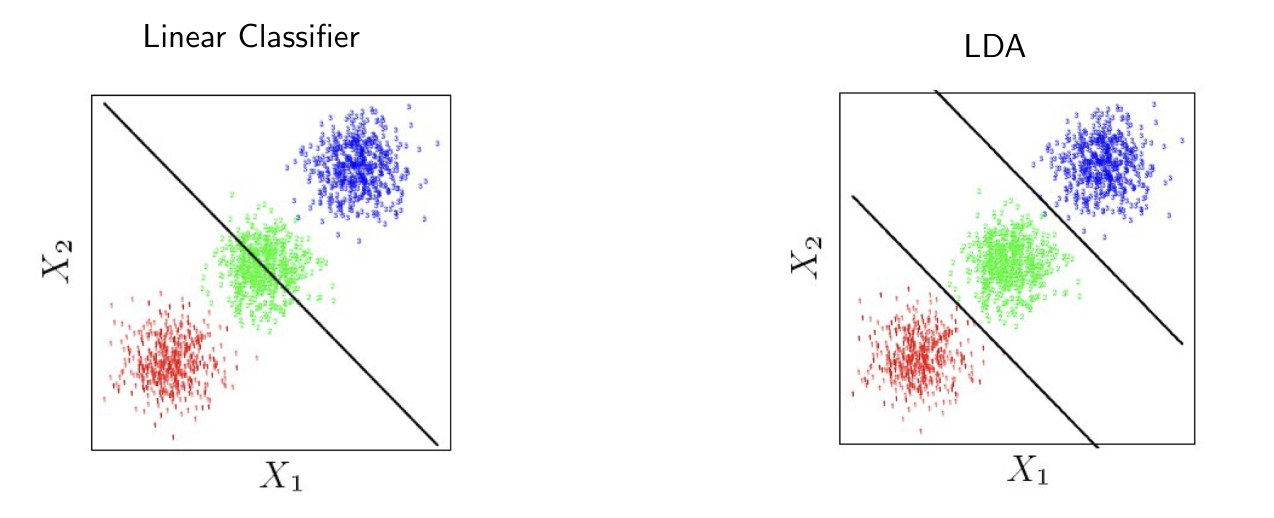
\includegraphics[width=0.5\linewidth]{Images/bayes_linear/LDA.png}
    \caption{Boundary Conditions LDA.}
\end{figure}

\subsection{Quadratic Discriminant Analysis}
Se durante la scelta della covarianza, si sceglie un modello diverso, è possibile ottenere un modello QDA, un modello non lineare. \\
Un modello LDA, risulta spesso più robusto, ma l’assunzione di linearità è spesso non rispettata nei casi reali. \\ 
Un modello QDA, invece è più dinamico, ma è più difficile controllare overfitting e altri problemi. \\ 

\begin{figure}[!htb]
    \centering
    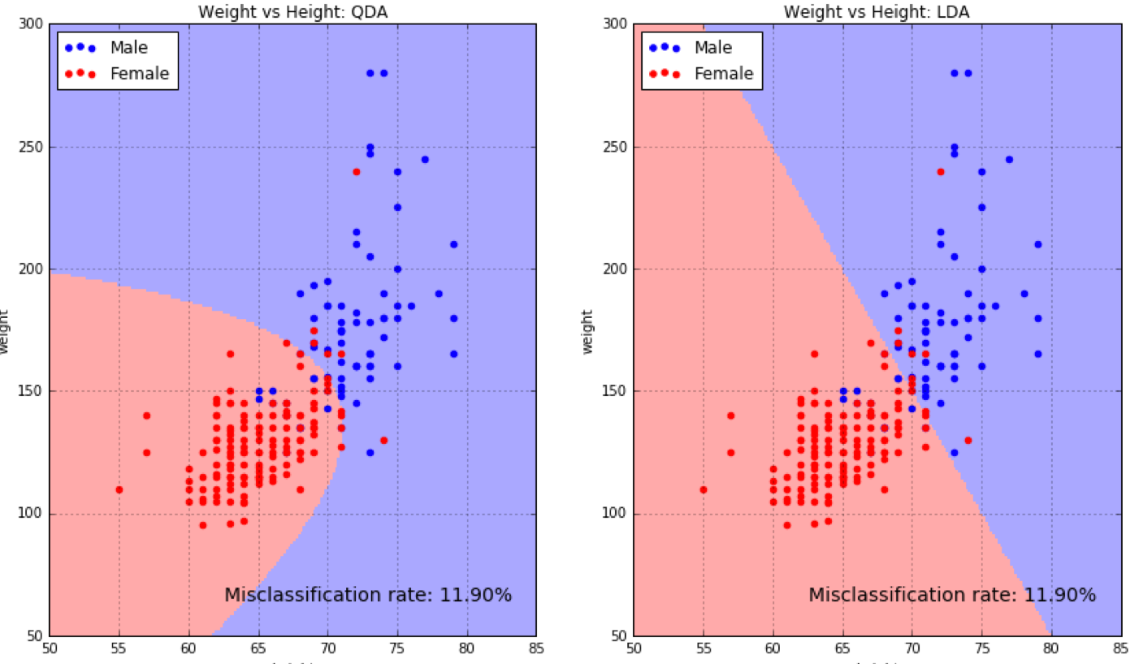
\includegraphics[width=0.5\linewidth]{Images/bayes_linear/LDA_QDA.png}
    \caption{Confronto fra LDA e QDA.}
\end{figure}

\begin{note}[Note Finali]
\begin{itemize}
  \item La dipendenza quadratica da $D$ rende l'LDA più lento del Naive Bayes di un fattore $D$, sia in fase di apprendimento che di classificazione.
  \item Il modello richiede $O(D^2C)$ parametri. Ciò può comunque rappresentare una buona compressione dei dati quando $D << N$. 
  \item In generale, la LDA richiederà più dati rispetto a Naive Bayes, poiché deve stimare i parametri $O(D^2)$ nella matrice di covarianza aggregata $\Sigma$.
\end{itemize}
\end{note}

\section{Logistic Regression}
La logistic regression è un classificatore discriminativo probabilistico A-Posteriori.
La sua funzione di classificazione è:
\[
  f_{LR}(x) = \arg\max_{c \in \mathcal{Y}} P(Y = c \mid x)
\]
Nel caso binario, modella direttamente la probabilità a posteriori come:
\[
  \begin{aligned}
    P(Y = 0 \mid x) &= \frac{e^{w^T x + b}}{1 + e^{w^T x + b}} \\
    P(Y = 1 \mid x) &= \frac{1}{1 + e^{w^T x + b}}
  \end{aligned}
\]
Calcolando le boundary conditions, si dimostra che il che è lineare. \\ 
C'è anche il caso con $K$ classi:
\[
  \begin{aligned}
    P(Y = c \mid x) &= \frac{\exp(w_c^T x + b_c)}{1 + \sum_{l=1}^{K-1} \exp(w_l^T x + b_l)} \\
    P(Y = K \mid x) &= \frac{1}{1 + \sum_{l=1}^{K-1} \exp(w_l^T x + b_l)}
  \end{aligned}
\]
\subsection{Ottimizzazione dei Parametri}
I parametri del modello di regressione logistica $\theta = \{(w_c, b_c), c \in \mathcal(y)\}$
vengono selezionati per ottimizzare la log likelyhood condizionata delle etichette dato un set di dati $D = \{(x_i, y_i), i = 1 : n\}$:
\[
  \theta_* = \arg\max_{\theta} \mathcal{L}(\theta \mid D) = \arg\max_{\theta} \sum_{i=1}^{n} \log P(Y = y_i \mid X = x_i)
\]
Tuttavia, la funzione $\mathcal{L}(\theta \mid D)$ non può essere massimizzata analiticamente. L'apprendimento dei parametri del modello richiede metodi di ottimizzazione numerica.

\subsection{Discesa del Gradiente}
\begin{defn}[Discesa del Gradiente]
  La discesa del gradiente è un algoritmo di ottimizzazione iterativo per trovare il minimo di una funzione.
  Eseguire un passo proporzionale all'opposto del gradiente della funzione nel punto corrente.
\end{defn}
Se consideriamo una funzione $f(\theta)$, l'\textbf{aggiornamento della discesa} del gradiente, per ogni parametro $\theta_j$, può essere espresso come:
\[
  \theta_j = \theta_j - \alpha \frac{d}{d\theta_j} f(\theta)
\]
La dimensione del passo è controllata dal \textbf{tasso di apprendimento} $\alpha$.
Scegliere il tasso di apprendimento $\alpha$ corretto è fondamentale per procedere correttamente verso il minimo:
\begin{itemize}
  \item Un passo troppo piccolo potrebbe portare a una convergenza estremamente lenta.
  \item Se il passo è troppo ampio, l'ottimizzatore potrebbe oltrepassare il minimo o addirittura divergere.
\end{itemize}

\begin{figure}[!htb]
    \centering
    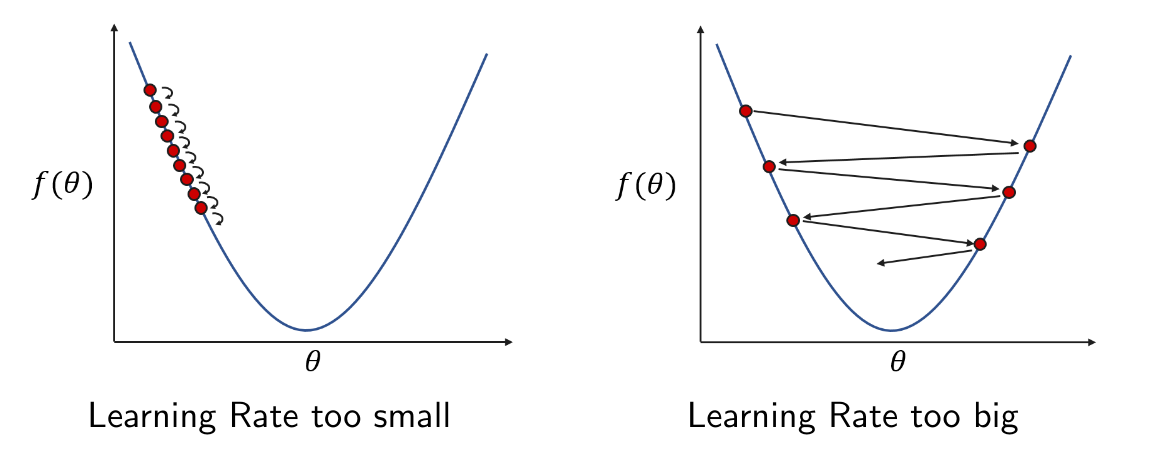
\includegraphics[width=0.5\linewidth]{Images/bayes_linear/Learning_Step.png}
    \caption{Scelta tasso di apprendimento.}
\end{figure}

Esistono diversi tipi di discesa del gradiente:
\begin{itemize}
  \item \textbf{Batch gradient descent:} ottimizzazione su l’intero batch di dati.
  \item \textbf{Mini batch stochastic gradient descent:} ad ogni step considero solo un piccolo insieme di dati, presi dal training set.
  \item \textbf{Stochastic gradient descent:} caso in cui per ogni step considero solo 1 esempio.
\end{itemize}

\begin{note}[Convessità]
  Se la funzione è convessa, la discesa del gradiente converge al \textbf{minimo globale}. Nel caso di funzioni non convesse, può convergere a \textbf{minimi locali}.
\end{note}

\begin{note}[Note Finali]
  \begin{itemize}
    \item In fase di classificazione, la LR è più veloce di NB e LDA. L'apprendimento della LR richiede un'ottimizzazione numerica, che risulta più lenta rispetto a NB.
    \item Richiede gli stessi parametri degli altri modelli (o meno se $C << D$).
    \item Ha più accuratezza in casi lineari con tante classi.
  \end{itemize}
\end{note}
